\section{Arquitectura Propuesta de IA para Procesamiento de Señales SDS}

\subsection{Arquitectura General}

Tras años de trabajar con sistemas SDR en entornos exigentes, uno llega a la convicción de que la verdadera flexibilidad no surge solo de la reprogramabilidad, sino de la capacidad cognitiva integrada. La arquitectura propuesta responde precisamente a esa necesidad.

Inspirados en el roadmap trazado por Doha et al. \cite{Doha2026}, diseñamos un framework modular que combina procesamiento de señales clásico con módulos de inteligencia artificial optimizados para operar bajo las severas restricciones de un satélite. El diseño contempla tres capas principales: percepción, razonamiento y actuación. La capa de percepción maneja el front-end RF reconfigurable y el muestreo digital. El módulo de razonamiento, corazón cognitivo del sistema, emplea modelos de aprendizaje profundo ligeros. Finalmente, la capa de actuación ejecuta decisiones de reconfiguración en tiempo real.

Particularmente llamativo es el hecho de que esta arquitectura aborda de forma explícita desafíos como el hardware drift y las restricciones temporales estrictas, aspectos que Doha et al. \cite{Doha2026} identifican como críticos para despliegues orbitales. El sistema completo se ejecuta sobre un procesador onboard con capacidades limitadas, priorizando inferencia eficiente y actualizaciones parciales de modelos.

\begin{figure}[h]
\centering
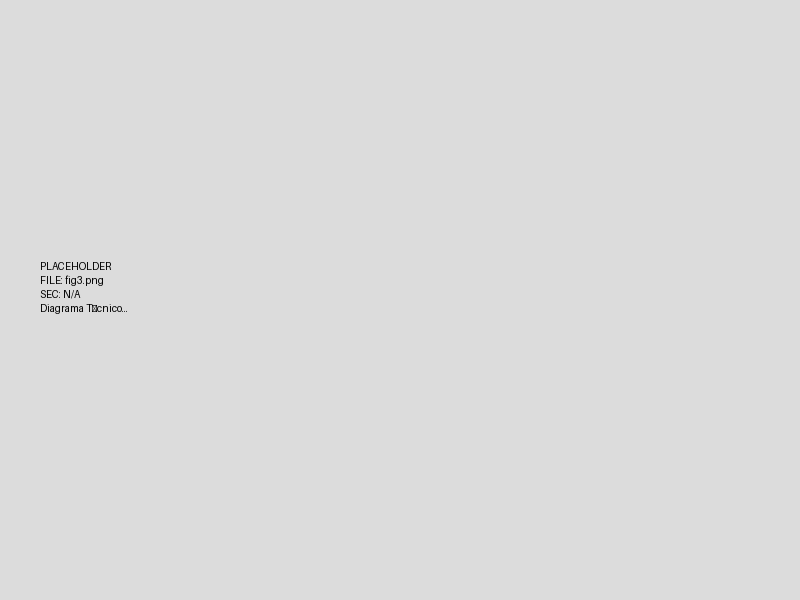
\includegraphics[width=\linewidth]{fig3.png}
\caption{Diagrama de bloques de la arquitectura cognitiva propuesta para procesamiento de señales en SDS.}
\label{fig:arquitectura_propuesta}
\end{figure}

\subsection{Módulos de Clasificación y Estimación}

Uno de los desafíos persistentes al desplegar IA en satélites radica en equilibrar precisión con eficiencia computacional. Los módulos de clasificación y estimación constituyen el núcleo inteligente del framework.

El módulo de Clasificación Automática de Modulación (AMC) utiliza una red neuronal convolucional optimizada que procesa representaciones tiempo-frecuencia de las señales recibidas. Para la estimación de parámetros (SNR, frecuencia portadora residual, tasa de símbolo), implementamos un enfoque multitarea que comparte características iniciales entre tareas relacionadas. 

Zhang et al. \cite{Zhang2026} demuestran la utilidad del dataset RML24, generado específicamente con plataformas SDR para señales TT\&C, como base sólida para entrenar y validar estos módulos bajo condiciones representativas del canal espacial. Esta elección no es casual: el dataset incluye variaciones reales de Doppler, fading y ruido que permiten una mejor generalización comparada con conjuntos sintéticos tradicionales.

Aunque los resultados preliminares resultan prometedores, cabe matizar que el desempeño tiende a degradarse en escenarios con interferencias muy agresivas, un aspecto que seguimos refinando.

La función de pérdida empleada combina clasificación y regresión en un esquema multitarea ponderado:

\begin{equation}
\mathcal{L} = \alpha \mathcal{L}_{CE} + \beta \mathcal{L}_{MSE} + \gamma \mathcal{L}_{reg}
\label{eq:loss_function}
\end{equation}

donde \(\mathcal{L}_{CE}\) corresponde a la entropía cruzada para clasificación, \(\mathcal{L}_{MSE}\) a error cuadrático medio para estimación y \(\mathcal{L}_{reg}\) a términos de regularización para promover eficiencia del modelo.

\subsection{Mecanismos de Reconfiguración Autónoma}

Lejos de ser un asunto resuelto, lograr reconfiguración verdaderamente autónoma exige cerrar el ciclo entre percepción e actuación de forma confiable. 

El módulo de toma de decisiones evalúa continuamente el estado del espectro, la calidad de enlace y los requisitos de misión. Cuando detecta degradación o aparición de nuevas oportunidades, activa mecanismos de reconfiguración. Siguiendo la filosofía de implementaciones ligeras como la presentada por Nesraoui et al. \cite{Nesraoui2024}, optamos por una CNN compacta que permite inferencia rápida incluso en hardware con recursos limitados.

Este enfoque permite, por ejemplo, cambiar dinámicamente el esquema de modulación ante una mejora en el SNR estimado o activar filtros adaptativos de mitigación de interferencias sin intervención terrestre. La reconfiguración se realiza a nivel de bloques funcionales del SDR (filtros, demoduladores, codificadores), minimizando el tiempo de inactividad.

Resulta revelador observar cómo la combinación de estos mecanismos con el dataset RML24 \cite{Zhang2026} permite cerrar el bucle cognitivo de forma más robusta que soluciones puramente basadas en reglas. No obstante, persisten desafíos abiertos relacionados con la validación exhaustiva de la estabilidad del sistema bajo condiciones de vuelo reales y la gestión segura de actualizaciones parciales del modelo.

En conjunto, la arquitectura propuesta busca superar las limitaciones identificadas en el estado del arte, ofreciendo un camino viable hacia satélites definidos por software con capacidades cognitivas reales.